\section{Redes neuronales profundas}

TODO

\subsection{Redes neuronales convolucionales}

\noindent
En 1989, el francés Yann LeCun comenzó a trabajar en los fundamentos de un novedoso modelo\
neuronal basado en la biología de la corteza visual del cerebro animal. Su trabajo, eventualmente\
lo llevó a ser nombrado director de la investigación en IA en Facebook. Pero más allá de su ascenso\
al \emph{``podio''} del aprendizaje profundo, su trabajo ha provocado una revolución en el\
\emph{estado del arte} del reconocimiento de imágenes a través de computadoras. Y lo más probable\
es que el mismo modelo continúe sobresaliendo por algunos años.\par
Como la mayoría de las arquitecturas neuronales, las \textbf{redes neuronales convolucionales}\
(\emph{CNN's}, por sus siglas en inglés) no alcanzaron la popularidad suficiente hasta entrada\
la época reciente, caracterizada por una alta conectividad (a través de Internet) y un incremento\
significativo en la capacidad de cómputo de los dispositivos modernos. Sin embargo, LeCun ya había\
obtenido resultados sobresalientes hacía 1998, en tareas de reconocimiento de patrones \cite{bengio2009}.\
El enfoque de LeCun, y de su equipo en \emph{Bell Labs}, consistió en dar un modelo de mayor\
capacidad en \emph{representaciones internas} que el tradicional perceptrón multicapa.\par
Un aspecto importante en esta arquitectura trata sobre la delegación de ciertas partes de la misma\
a sub-problemas específicos de la tarea a resolver. Por consiguiente, cada capa de una CNN definirá\
uno (o varios) niveles de representación, los cuales abstraen ciertas características inherentes\
al flujo de datos de entrada. Mediante un basto conjunto etiquetado de datos, se pueden aprender dichas\
abstracciones de manera supervisada.

\subsubsection*{La capa convolucional}

La filosofía \emph{reduccionista} de la ciencia, que es la que sigue dando sustento a diversos métodos\
de trabajo de distintas disciplinas, sugiere que al estudiar a un objeto o fenómeno, se haga de manera\
modular, empezando por las estructuras más básicas que lo componen hasta \emph{``el todo''}. Ello supone\
una jerarquía de fragmentos, con atributos bien definidos y una especie de \emph{función}, cuyo rol\
es el de componer todos los fragmentos en uno. Asimismo, la idea de una jerarquía de características\
conduce a la arquitectura convolucional, de la misma manera con la que una persona identifica parte por\
parte lo que sucede en una imagen.\par
Para iniciar la discusión sobre la estructura de una CNN, usaremos como ejemplo al reconocimiento\
computacional de imágenes; sin embargo, cabe notar que esta arquitectura es popular en tareas donde\
exista la necesidad de reconocer patrones y sobre conjuntos de datos con topología \emph{cuadriculada}.\
\footnote{De acuerdo a \cite{goodfellow-et-al-2016}, como ejemplos de datos con una topología cuadriculada,\
  se incluyen series de tiempo (cuadrícula de una dimensión), audio o videos.}
Uno de los conjuntos de datos más famosos, y de mayor tradición, es la \emph{Mixed National Institute of Standards}\
\emph{and Technology database}, mejor conocida como MNIST. En ella se alberga una gran cantidad de dígitos\
escritos a mano; el problema, entonces, consiste en clasificar cualquier manuscrito dado en una de las $10$ clases\
existentes, de acuerdo al dígito más parecido.\par

\begin{figure}
  \centering
  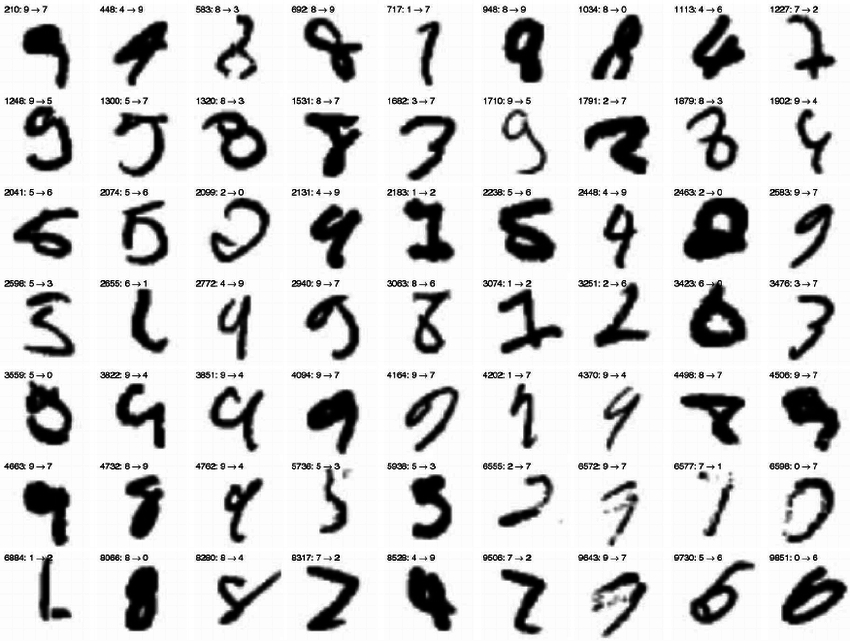
\includegraphics[width=0.6\textwidth]{mnist}
  \caption{Algunos dígitos existentes en la base de datos MNIST.
    (Tomado de \url{http://www.researchgate.net/}.)}
  \label{mnist_fig}
\end{figure}

Como se observa en la figura (\ref{mnist_fig}), existen distintas maneras de escribir un solo dígito. Quisiéramos\
que nuestra solución sea lo suficientemente robusta para distinguir $4$'s de $9$'s por más ilegible que\
sea la letra. No tenemos idea de dónde buscar ciertas características o si el observar un cambio drástico\
en el color de varios pixeles contiguos nos sea significativo; todo esto es parte de lo que se deberá de\
\emph{aprender}. Esta incertidumbre en la detección de atributos conduce a, de alguna manera, ir en\
búsqueda de pequeñas porciones de la imagen que nos den una pista por dónde empezar.\par
En este punto cabe recordar que usualmente para una computadora, una imagen es un arreglo de tres dimensiones,\
cada una especificando la posición de un pixel y su color. En la práctica (y de acuerdo a las últimas tendencias\
de programación de redes neuronales), a esta estructura se le llama \textbf{tensor}, por lo que seguiremos\
la convención. Volviendo a nuestra búsqueda, necesitamos un parámetro que nos indique el mínimo de pixeles a\
analizar para empezar a encontrar detalles claves de la imagen. Por ello, vamos a usar un pequeño tensor\
para recorrer toda la imagen e ir desvelando patrones claves. A dicho tensor le llamaremos \textbf{filtro}\
(\emph{kernel}, en inglés) y a su dimensión, \textbf{zancada} (\emph{stride}, en inglés)\par
Matemáticamente, este proceso se puede formalizar mediante la convolución de dos funciones reales.\
Si $x$ denota a nuestro dígito desconocido y $w$ a nuestro filtro, entonces la convolución de $x$ con\
$w$, en un punto $t$, se define como:
\begin{equation}
  c(t) := \int x(a) w(t-a) da
\end{equation}
y se denota:
\begin{equation}
  c(t) = (x * w)(t).
\end{equation}
En el mundo digital, tenemos conjuntos de datos discretos, por lo que es conveniente dar una definición\
adaptada al respecto:
\begin{equation}
  c(t) = (x * w)(t) := \sum _{a=-\infty} ^{\infty} x(a) w(t-a).
\end{equation}
Dentro del contexto de reconocimiento de imágenes, es útil especificar que la convolución se hace en dos\
dimensiones de las que se están contemplando. Para ello introducimos la siguiente notación:\
si $i$ y $j$ son valores que denotan la posición de un pixel, $X(i,j)$ es el valor (color) correspondiente\
y $K(i,j)$ denota la entrada $(i,j)$ de nuestro filtro, definimos a la convolución $C$ como:
\begin{equation}
  C(t) = (K * I)(i,j) := \sum_m \sum_n I(i-m,j-n) K(m,n).
\end{equation}
Muchas bibliotecas de redes neuronales utilizan la \textbf{correlación cruzada} en vez de la convolución.\
Semánticamente, la correlación cruzada sirve para analizar lo mismo que buscamos con la convolución; por\
ello, esta sutil distinción muchas veces no es notada. La definición es la siguiente:
\begin{equation} \label{cross_corr}
  C(t) = (I * K)(t) := \sum_m \sum_n I(i+m,j+n) K(m,n).
\end{equation}
Nótese que en las dos últimas definiciones se ha convenido \emph{voltear} los índices del filtro. En la\
teoría, la ventaja que trae esto consiste en una mayor facilidad de probar ciertos resultados.\par
Para terminar de describir a lo que se le conoce como la \textbf{capa convolucional} de la arquitectura,\
vale la pena hablar un poco sobre la salida de (\ref{cross_corr}). De hecho, en realidad tenemos muchas salidas que\
son resultado de multiplicar partes de la imagen de entrada con el filtro. (El producto de matrices usado\
en este caso se efectúa \emph{entrada por entrada} y no como se acostumbra.) A los tensores resultantes\
se les conoce, convenientemente, como \textbf{mapas de características}.\par
Aquí cabe señalar que la eficiencia de la convolución es mucho mayor a la de una\
multiplicación de matrices (en una capa densa) y esto ocurre, principalmente, por las siguientes razones:
\begin{itemize}
\item En una capa densa, se consideran interacciones entre cada neurona de entrada con cada neurona de salida.\
  Es decir, los productos matriciales involucran a cada pixel, sin importar qué lugares en específico son\
  los que vale la pena resaltar.
\item Se dice que en una capa convolucional se manejan \textbf{pesos esparcidos}, los cuales corresponden\
  a las entradas del filtro. Esto implica que después de un entrenamiento, el filtro aprenderá a interactuar\
  con ciertos grupos de pixeles, sin conocer su distribución.
\item En una capa convolucional, los pesos del filtro que se buscan aprender son mucho menos que los pesos que\
  se aprendería en una capa densa: si la imagen de entrada contiene miles o millones de pixeles, entonces\
  necesitamos cientos de pixeles en nuestro filtro para aprender los razgos más pequeños de la misma (como\
  bordes o puntos).
\end{itemize}\par
En resumen, si tenemos $m$ entradas y $n$ salidas en una capa, y ésta es densa, entonces habremos de realizar\
$O(m \times n)$ operaciones para calcular la salida. En cambio, en una capa convolucional, podemos tener\
una zancada $k$ de pixeles en el filtro, con un orden de magnitud mucho menor a $n$; lo cual va a provocar\
que sea más eficiente calcular $O(m \times k)$ operaciones.\par
Como sucede al calcular las salidas de una capa densa, aquí hay que utilizar una función no lineal (y \emph{suave}) para\
finalizar la clasificación. En algunos casos, a este paso se le suele llamar \textbf{capa de no linealidad}.\
En \cite{lecun2010}, además de usar dicho término, se propone a la función $tanh$, sobre cada entrada de los\
mapas de características, como el estándar en CNN's. Sin embargo, también se señala que una \emph{sigmoide}\
\emph{rectificada} ha dado buenos resultados en reconocimiento de imágenes (sujeta a una normalización posterior);\
el caso particular es el de la \textbf{unidad lineal rectificada} (\emph{ReLU}, por sus siglas en inglés):
\begin{equation}
  f(x) = \max(0, x).
\end{equation}

\begin{figure}
  \centering
  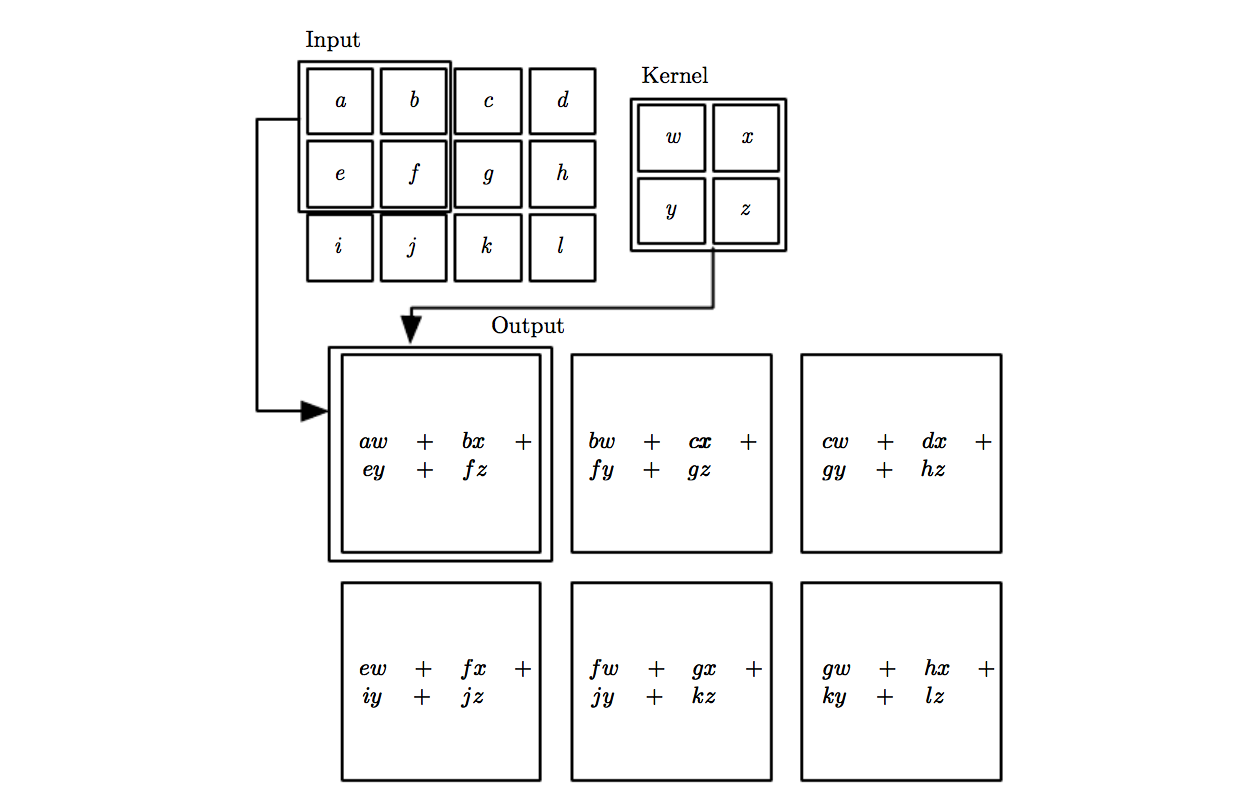
\includegraphics[width=0.9\textwidth]{2dconv}
  \caption{Ilustración del proceso de convolución. El filtro se desliza por la imagen de entrada y
    se efectúa un producto pixel por pixel.)
    (Tomado de \cite{goodfellow-et-al-2016}.)}
  \label{2dconv_fig}
\end{figure}

\subsubsection*{La capa de \emph{pooling}}

Un exceso de aprendizaje en la capa de convolución puede provocar un \emph{sobreajuste} sobre\
el modelo. Esto se puede observar, en nuestro ejemplo, con una arquitectura donde cada filtro\
se entrene a funcionar para un grupo pequeño y exclusivo de pixeles, los cuales esperen encontrar\
detalles claves en lugares precisos. Es necesario, entonces, ocuparse de que una CNN\
\emph{generalice} suficientemente su aprendizaje para aumentar su robustez.\par
Por ello, las CNN's llevan, además de capas convolucionales, algunas capas de \textbf{agrupación}\
(\emph{pooling}, en inglés y usaremos esta palabra en adelante) con las cuales se puede extraer\
los detalles más fundamentales de cada mapa de características. En la práctica, existen dos operaciones\
de pooling que sobresalen sobre las demás: \emph{max}-pooling y \emph{avg}-pooling. Para calcular cualquier\
capa de pooling, se define una vecindad en cada mapa de características (que no exceda su zancada);\
acto seguido, dependiendo del pooling a usar, se almacena el máximo o el promedio de los pixeles\
abarcados en la vecindad.\par
Con esta capa, la arquitectura convolucional se vuelve \textbf{aproximadamente invariante} a modificaciones\
en la entrada. A raíz del pooling, hay manera de disminuir los cómputos al menor númeor de neuronas\
brindando la posibilidad de optimizar mucho más la memoria utilizada y las dimensiones de las capas.

\begin{figure}
  \centering
  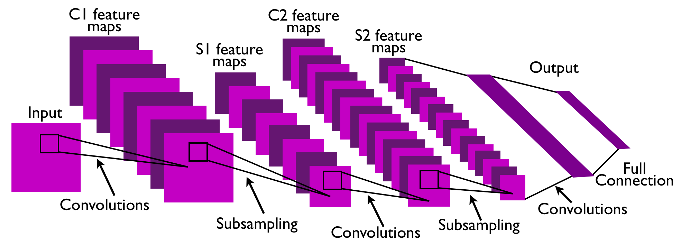
\includegraphics[width=0.8\textwidth]{convnet}
  \caption{Estructura básica de una red neuronal convolucional, con dos fases de extracción de características.
    (Tomado de \cite{lecun2010})}
  \label{convnet_fig}
\end{figure}

\subsubsection*{Entrenamiento}

TODO


\subsection{Redes neuronales recurrentes}

TODO


\subsubsection*{LSTM's}

TODO


\subsubsection*{¿Cómo funciona la arquitectura recurrente?}

TODO


\subsubsection*{Entrenamiento}

TODO
